\documentclass{beamer}
\usetheme{Warsaw}

\usepackage{graphicx} % Allows including images
\usepackage{booktabs} % Allows the use of \toprule, \midrule and \bottomrule in tables
\usepackage{listings}
\usepackage[utf8]{inputenc}
\usepackage[overlay,absolute]{textpos}
\usepackage{amsfonts}

\AtBeginSection[]
{
\begin{frame}<beamer>
\frametitle{Plan}
\tableofcontents[
  currentsection,
  hideothersubsections
]
\end{frame}
}

\lstset{language=C++,
                basicstyle=\ttfamily,
                keywordstyle=\color{green}\ttfamily,
                stringstyle=\color{red}\ttfamily,
                commentstyle=\color{cyan}\ttfamily,
                morecomment=[l][\color{magenta}]{\#},
                escapechar=@
}

\setbeamercolor{normal text}{fg=white,bg=black!90}
\setbeamercolor{structure}{fg=white}

\setbeamercolor{alerted text}{fg=red!85!black}

\setbeamercolor{item projected}{use=item,fg=black,bg=item.fg!35}

\setbeamercolor*{palette primary}{use=structure,fg=structure.fg}
\setbeamercolor*{palette secondary}{use=structure,fg=structure.fg!95!black}
\setbeamercolor*{palette tertiary}{use=structure,fg=structure.fg!90!black}
\setbeamercolor*{palette quaternary}{use=structure,fg=structure.fg!95!black,bg=black!80}

\setbeamercolor*{framesubtitle}{fg=white}

\setbeamercolor*{block title}{parent=structure,bg=black!60}
\setbeamercolor*{block body}{fg=black,bg=black!10}
\setbeamercolor*{block title alerted}{parent=alerted text,bg=black!15}
\setbeamercolor*{block title example}{parent=example text,bg=black!15}

\author[Félix-Antoine Ouellet]{Félix-Antoine Ouellet}

\title[PGAS\hspace{2em}\insertframenumber/\inserttotalframenumber]{Espace d'addressage global partitionné}

\institute{Université de Sherbrooke}

\date{2 octobre 2014}

\begin{document}

\begin{frame}
\titlepage % Print the title page as the first slide
\end{frame}

\begin{frame}
\tableofcontents[hideallsubsections]
\end{frame}

\section{Motivation}
\subsection{État présent du matériel}
\begin{frame}
\frametitle{Explosion de parallélisme}
\framesubtitle{Appareils courants}
\begin{itemize}
\item Processeurs vectoriels
\item Processeurs multi-coeurs
\item Accélérateurs
\end{itemize}
\end{frame}

\begin{frame}
\frametitle{Explosion de parallélisme}
\framesubtitle{Superordinateurs}
\begin{itemize}
\item Aux portes de l'\textit{exascale computing}
\item<2-> $10^{18}$ opérations en virgule flottante par seconde
\item<3-> Potentiellement 1 milliard de \textit{threads} à gérer simultanément
\item<4-> Pas nécessairement utiliser par des informaticiens
\end{itemize}
\end{frame}

\subsection{État présent du logiciel}
\begin{frame}
\frametitle{Programmation parallèle avec mémoire partagée}
\begin{center}
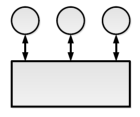
\includegraphics[scale=3]{shared.png}
\end{center}
\end{frame}

\begin{frame}
\frametitle{Programmation parallèle avec mémoire partagée}
\begin{minipage}[t]{0.5\linewidth}
    \textbf{Avantages}:
    \begin{itemize}
    \item{Raisonnement plus facile}
    \item{Unique espace d'addressage}
    \end{itemize}
    \end{minipage}%
    \begin{minipage}[t]{0.5\linewidth}
    \textbf{Inconvénients}:
    \begin{itemize}
    \item{Conditions de course}
    \item{N'échelonne pas bien}
    \end{itemize}
\end{minipage}
\end{frame}

\begin{frame}
\frametitle{Programmation parallèle avec mémoire distribuée}
\begin{center}
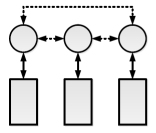
\includegraphics[scale=3]{distributed.png}
\end{center}
\end{frame}

\begin{frame}
\frametitle{Programmation parallèle avec mémoire distribué}
\begin{minipage}[t]{0.5\linewidth}
    \textbf{Avantages}:
    \begin{itemize}
    \item{S'échelonne bien}
    \item{Pas de conditions de course}
    \end{itemize}
    \end{minipage}%
    \begin{minipage}[t]{0.5\linewidth}
    \textbf{Inconvénients}:
    \begin{itemize}
    \item{Doit penser à la distribution des données}
    \item{Performance lié au réseau}
    \end{itemize}
\end{minipage}
\end{frame}

\begin{frame}
\frametitle{Programmation parallèle}
\begin{itemize}
\item Des abstractions de trop bas niveau nuisent à la productivité
\item Des abstractions de trop haut niveau nuisent à la performance
\end{itemize}
\end{frame}

\section{Espace d'addressage global partitionné}
\begin{frame}
\frametitle{Espace d'addressage global partitionné}
\begin{center}
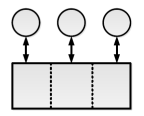
\includegraphics[scale=3]{pgas.png}
\end{center}
\end{frame}

\subsection{Programmation à haut niveau}
\begin{frame}
\frametitle{Programmation à haut niveau}
\begin{itemize}
\item L'espace d'addressage apparaît unifié
\item Peu de notions de parallélisme
\item Le compilateur s'occupe de faire marcher le tout
\end{itemize}
\end{frame}

\begin{frame}[fragile]
\frametitle{Programmation à haut niveau}
\framesubtitle{Exemple}
\begin{lstlisting}
Vector<int> Add(Vector<int> A, 
                Vector<int> B) {
  Vector<int> C;
  @\textcolor{green}{parfor}@(int i = 0; i < 100000000; ++i) {
    C[i] = A[i] + B[i];  
  }
  
  return C;
}
\end{lstlisting}
\end{frame}

\begin{frame}
\frametitle{Programmation à haut niveau}
\begin{itemize}
\item Pas nécessairement la version optimale qui sera produite
\item Par contre, il s'agit de la version qui maximise la productivité
\end{itemize}
\end{frame}

\subsection{Localité}
\begin{frame}
\frametitle{Localité}
\begin{itemize}
\item Faire la distinction entre ce qui est global et ce qui est local
\item Contrôler la distribution des données
\begin{itemize}
\item<2-> Profiter des hiérarchies mémoire modernes
\item<2-> Profiter de divers types de processeurs
\end{itemize}
\end{itemize}
\end{frame}

\begin{frame}[fragile]
\frametitle{Localité}
\framesubtitle{Code}
\begin{lstlisting}
@\textcolor{green}{global}@ Vector<int> Vec;
@\textcolor{green}{global}@ int TotalSum
/*...*/
for(int i = 0; i < nbLocales(); ++i) {
  do @\textcolor{green}{on}@ Locale[i] {
    int PartialSum = 0;
    for(int j = 0; j < ; ++j)
       PartialSum += Vec[j];
    TotalSum += PartialSum;
  }
}
\end{lstlisting}
\end{frame}

\subsection{Tâches}
\begin{frame}
\frametitle{Tâches}
\framesubtitle{Les bases}
\begin{itemize}
\item Ensemble d'instructions à exécuter
\item Repose sur un \textit{thread pool}
\item Possiblement lié à une localité
\end{itemize}
\end{frame}

\begin{frame}[fragile]
\frametitle{Tâches}
\framesubtitle{Les bases}
\begin{lstlisting}
void Func() {
  int Res = CalculComplexe(@\textcolor{green}{this\_locale}@.ID);
  print("Resultat:", Res);
}
/*...*/
for(int j = 0; j < nbLocales(); ++j) {
  do @\textcolor{green}{on}@ Locale[j] {
    Func();
  }
}
\end{lstlisting}
\end{frame}

\begin{frame}
\frametitle{Tâches}
\framesubtitle{Fonctionnalités avancées}
\begin{itemize}
\item Exploiter le calcul asynchrone
\item Créer dynamiquement des tâches
\item Invoquer des tâches situées sur une autre localité
\end{itemize}
\end{frame}

\begin{frame}[fragile]
\frametitle{Tâches}
\framesubtitle{Fonctionnalités avancées}
\begin{lstlisting}
void Func() {
  int Res = 0;
  @\textcolor{green}{parfor}@(int i = 0; i < 100; ++i)
    Res += CalculComplexe(@\textcolor{green}{this\_locale}@.ID);
  println("Locale:", @\textcolor{green}{this\_locale}@.ID);
  println("Resultat:", Res);
}
/*...*/
do @\textcolor{green}{on}@ Locale[3] {
    @\textcolor{green}{async}@ Func();
}
println("Locale:", @\textcolor{green}{this\_locale}@.ID);
\end{lstlisting}
\end{frame}

\section{Implémentation}
\begin{frame}
\frametitle{DARPA HPCS}
\begin{itemize}
\item \textit{High Productivity Computing Systems}
\item But: Produire des systèmes informatiques hautement productif pour l'industrie et la sécurité nationale
\end{itemize}
\end{frame}

\begin{frame}
\frametitle{Chapel}
\framesubtitle{Présentation}
\begin{itemize}
\item Réponse de Cray au projet HPCS
\item Inspiré de langage comme C, C++, C\#, Java, Fortran, HPF
\end{itemize}
\end{frame}

\begin{frame}[fragile]
\frametitle{Chapel}
\framesubtitle{Exemple - Calcul de PI}
\begin{lstlisting}
const numRect = 10000000;
const D : domain(1) = 1..numRect;
const width = 2.0 / numRect;
const baseX = -1 - width/2;
@\textcolor{green}{proc}@ rectangleArea(i : int) {
  const x = baseX + i*width;
  return width * sqrt(1.0 - x*x);
}
@\textcolor{green}{var}@ halfPI : @\textcolor{green}{real}@;
for i in D {
  halfPI += rectangleArea(i);
}
writeln("Result:",2*halfPI);  
\end{lstlisting}
\end{frame}


\section{Conclusion}
\begin{frame}
\frametitle{Conclusion}
\begin{itemize}
\item Les nouveaux défis en calcul de haute performance demande de nouvelles réponses
\item<2-> L'avènement de l'ère multi-coeurs va forcer les langages de programmation à évoluer
\end{itemize}
\end{frame}

\end{document}